\section{DVI encoder}

\marginpar{Include formula for exact throughput, and pixel clocks used for OV7670}

The \gls{dvi} encoder and decoder presented here are based heavily upon a reference design provided by Diligent's IP library for the Zybo development board. Rather than reinvent the wheel, this project opts to use these cores as a base and extend them for use with image sensors. All third-party code has been attributed, as per the BSD-license which the IP is released under. Custom additions have been commented.

\subsection{\texttt{rgb2dvi} module overview}

\begin{figure}
  \centering
  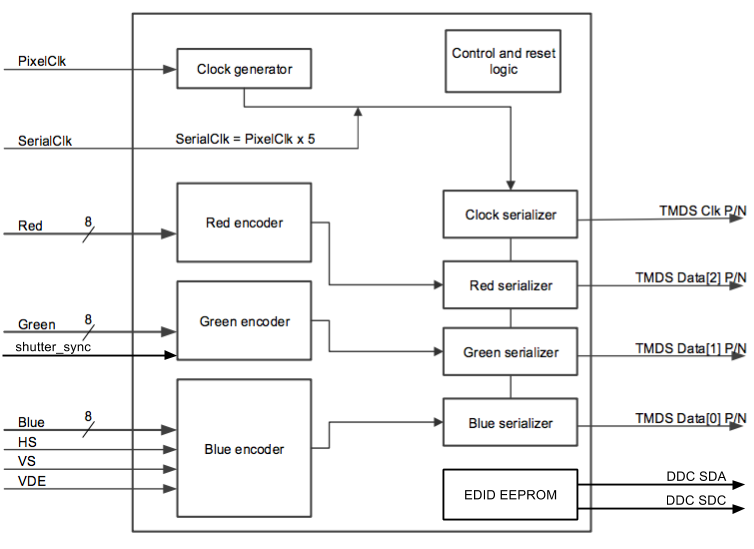
\includegraphics[width=1\textwidth]{./img/rgb2dvi.png}
  \caption{High-level overview of the image processor inside the camera body.}
  \label{fig:image_processor_diagram}
\end{figure}

The \gls{dvi} encoder takes a 24-bit wide pixel data bus as the main input, splitting off into three 8-bit channels for Red, Green and Blue. As the application requires a RAW pixel format instead of RGB we must deviate from the \gls{dvi} specification slightly by combining all channels into one large input, however internally they are still treated separately. Only a single channel (Blue) is used for data in the proof-of-concept as the OV7670 only has an 8-bit \gls{adc}, however the Green channel is also used to transmit the control signals related to flash and shutter synchronisation. Combining all channels gives a maximum pixel depth of 24-bits --- the image sensor on a professional \gls{dslr} will typical have a 12--14-bit \gls{adc}, so 24-bits is more than sufficient. Alongside the pixel bus are the regular video timing and synchronisation signals used elsewhere in the design. 

Internally the \gls{dvi} encoder instantiates three identical \texttt{TMDS\_encoder} blocks and assigns each one to a channel. Immediately after each \gls{tmds} encoder is an \texttt{OutputSERDES} block which is what actually drives the \gls{tmds}-encoded data across the interface. 

DDC channel

Flash sync

\subsection{TMDS encoding}

TMDS flow chart

VSYNC + HSYNC sent over control channel

\subsection{Serialisation}

Chaining diagram

\subsection{Clocking}

MMCM

Pixelclock fed into serialisers

\subsection{Performance}